\chapter{FSGui}
\label{chap:fsgui}
This chapter will deal with the requirements specification, analysis, design and non-trivial implementation details of FSGui.

\section{Requirements Specification}
The requirements for FSGui are:
\begin{itemize}
	\item must be installed on the staff's desktop computers
	\item must run on unix and windows systems
	\item must be a TCP client to FSServer
	\item must not need installation, just download and double-clik
	\item must create, save, load, export command sequences
	\item must execute failsafe scritps
	\item must view graphical representation of the health status
\end{itemize}
In addition to these requirements, the following requirement was identified when the overall design was agreed upon:
\begin{itemize}
	\item must be able to retrieve a list of server scripts and execute them with custom arguments
	\item must be able to execute local scripts
	\item must have an auto\_lock option
	\item must indicate connection and lock state
	\item must indicate when the health status was last updated
\end{itemize}

\section{Analysis and design}
Lets go through the requirements one by one. For each requirement we will enhance the design to incorporate the requirement.

\textbf{Must be installed on the staff's desktop computers} \\
Trivial constraint

\textbf{Must run on unix and windows systems} \\
There exists a number of cross-platform GUI frameworks we could use like Java swing or Xulrunner.

Xulrunner is Mozilla's cross-platform and open source framework. Xulrunner has the advantage that it is very easy to build complex and appealing GUIs in no time. The disadvantage is that the framework takes up 20 MB of harddisk space and is not included on UNIX og Windows by default. Furthermore, it lacks some systemwise features like spawning new processes and executing console commands.

The advantage with Java is that it runs on most systems and once you have the java virtual machine installed it is fairly easy to just pack an executable jar file and run it with a double click.
The FSGui will be implemented in JAVA using the Swing Framework.

\textbf{Must be a TCP client to FSServer} \\
When the program starts the user must indicate the address and port of the FSServer.
With a 30 sec token timeout the user will experience lock errors often enough to be annoying. Therefore, it must be possible to set an autolock option. It must also be clear to the user whether the server is locked or not and whether a connection has been made to FSServer or not.

\begin{figure}[h!] \centering
	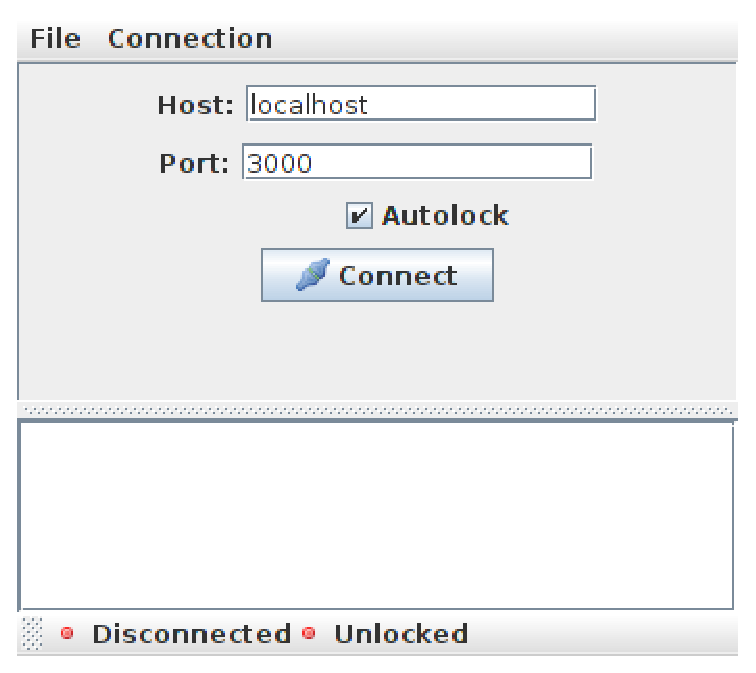
\includegraphics[scale=0.7]{img/fsgui_connect}
  \caption{The connect panel}
\end{figure}

\textbf{Must not need installation, just download and double-clik} \\
The FSGui will be packed as an executable jar file. The only requirement to the staff computers is that they have a Java Virtual Machine installed.

\textbf{Must send failsafe commands} \\
Java has built-in support for sockets and TCP.

\textbf{Must create, save, load and export command sequences} \\
For easy and fast testing, simple command sequences can be composed in the GUI. There are no conditionals or loops and the sequence will stop executing if one of the commands fails for one reason or another. It is possible to save and load sequences and to export a sequence to a Ruby script.

Sequences can be saved, loaded and exported to scripts.

\begin{figure}[h!] \centering
	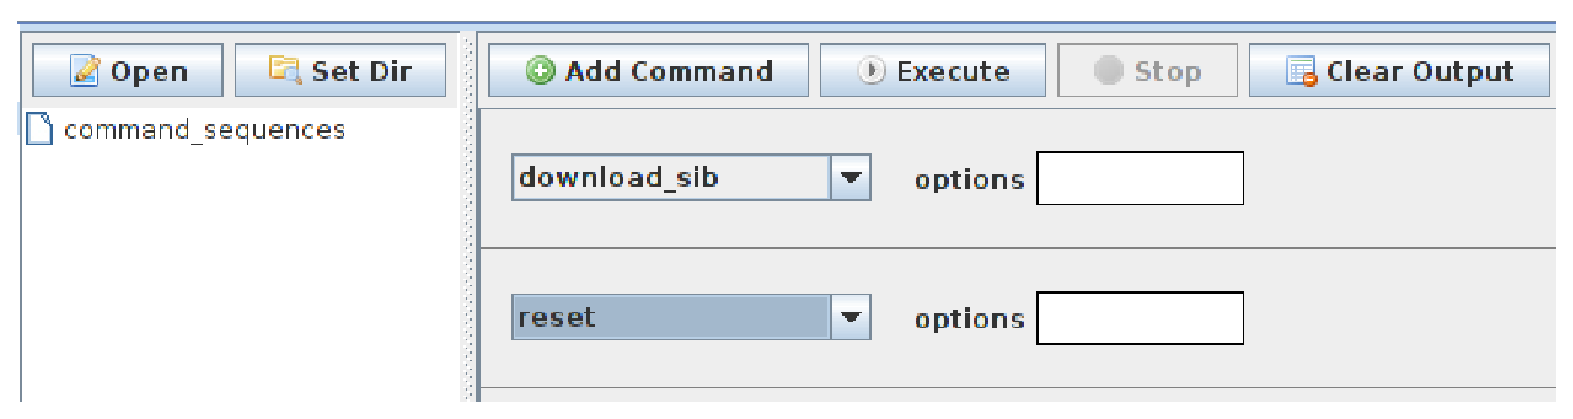
\includegraphics[scale=0.7]{img/fsgui_sequences}
  \caption{Command Sequences}
\end{figure}

\textbf{Must view graphical representation of the health status} \\
The satellite can read various health information from the individual subsystems and send them back to earth. Which data the subsystems will actually yield and how that data should be interpreted is not agreed upon as of this writing.

Instead the development board, that was used in place of the real satellite, simulates this data by reading several voltages and currents. When the real data is available the staff should be able to modify the source code of this project and fairly quickly replace the development data with the real data.

\begin{figure}[h!] \centering
	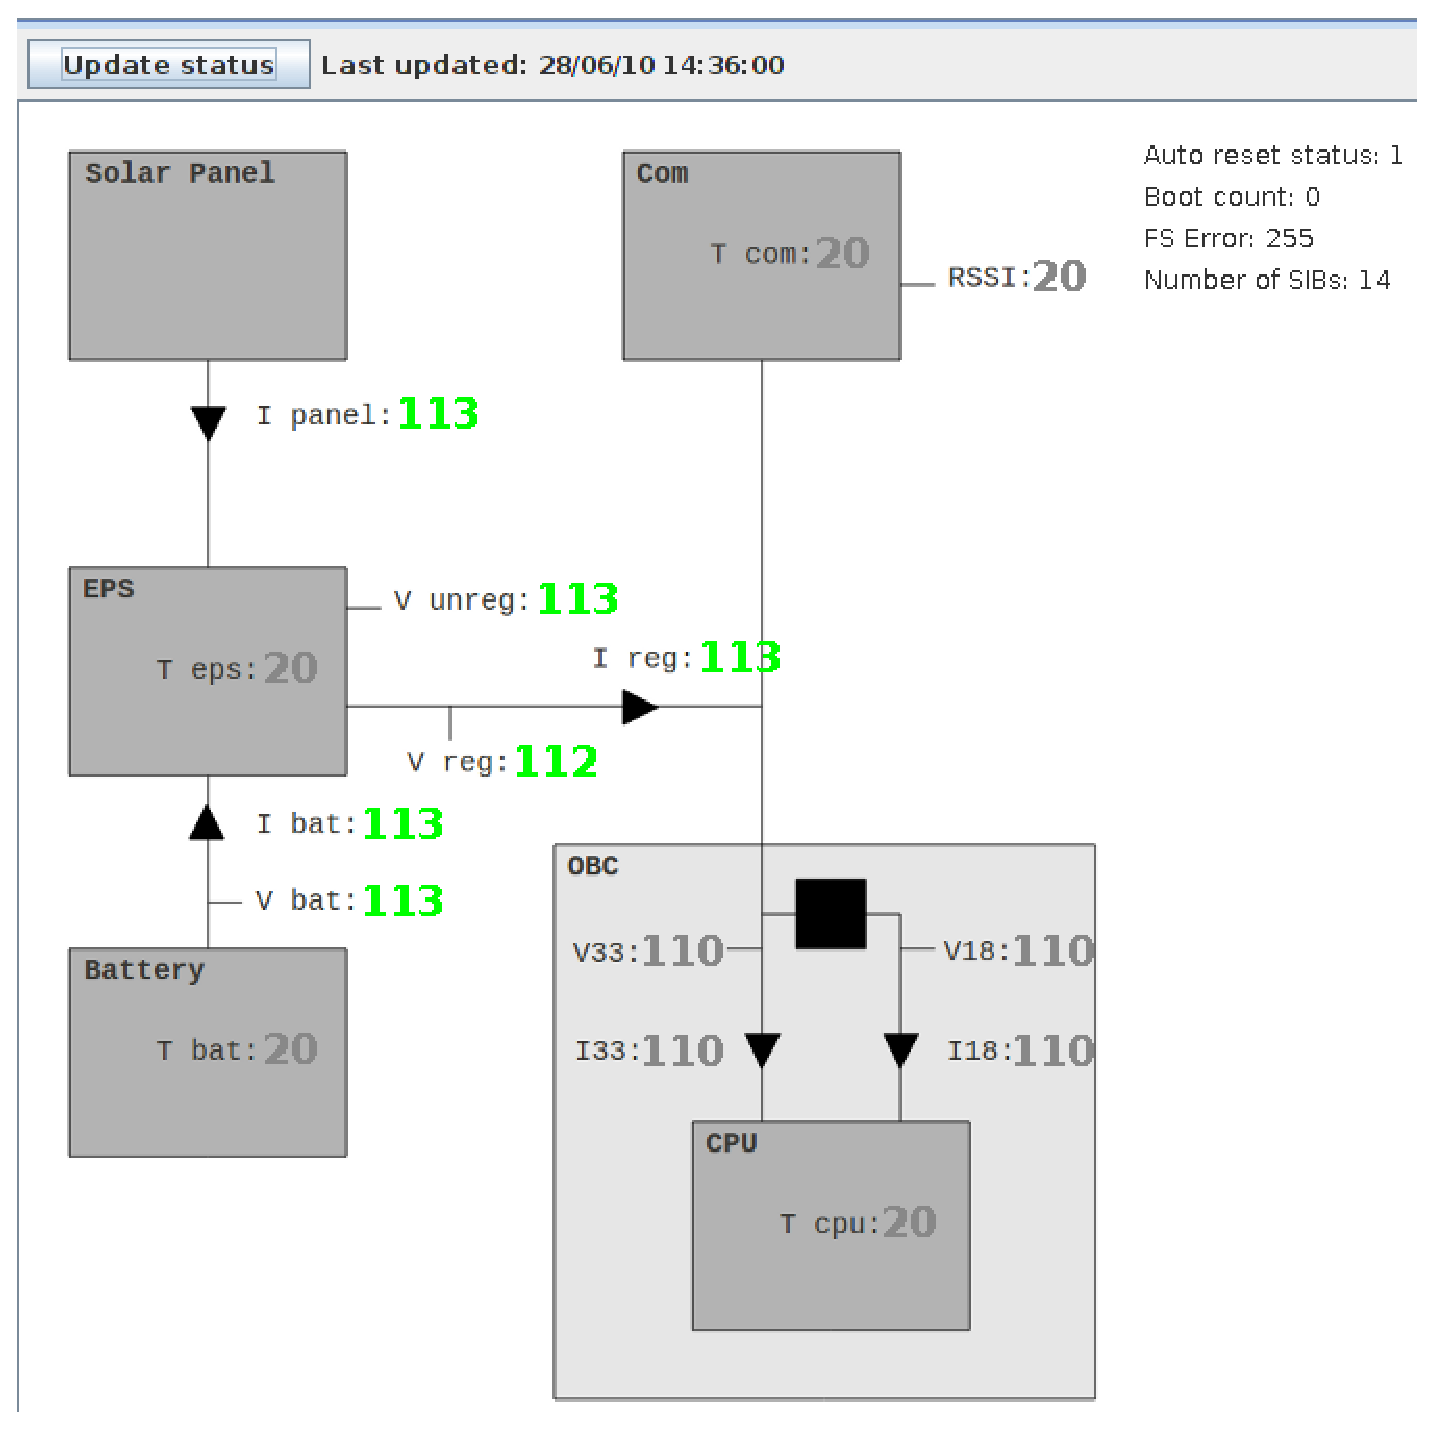
\includegraphics[scale=0.7]{img/fsgui_health}
  \caption{The Health Status with last updated stamp}
\end{figure}

\textbf{Must be able to execute local scripts} \\
In addition to running a script in the console it should also be possible to run and see the output of that script from within the GUI. The scripts are organized in a filetree and the user should be able to set the root of the filetree, navigate through the filetree, selecting a script, passing arguments to it and executing it.

\begin{figure}[h!] \centering
	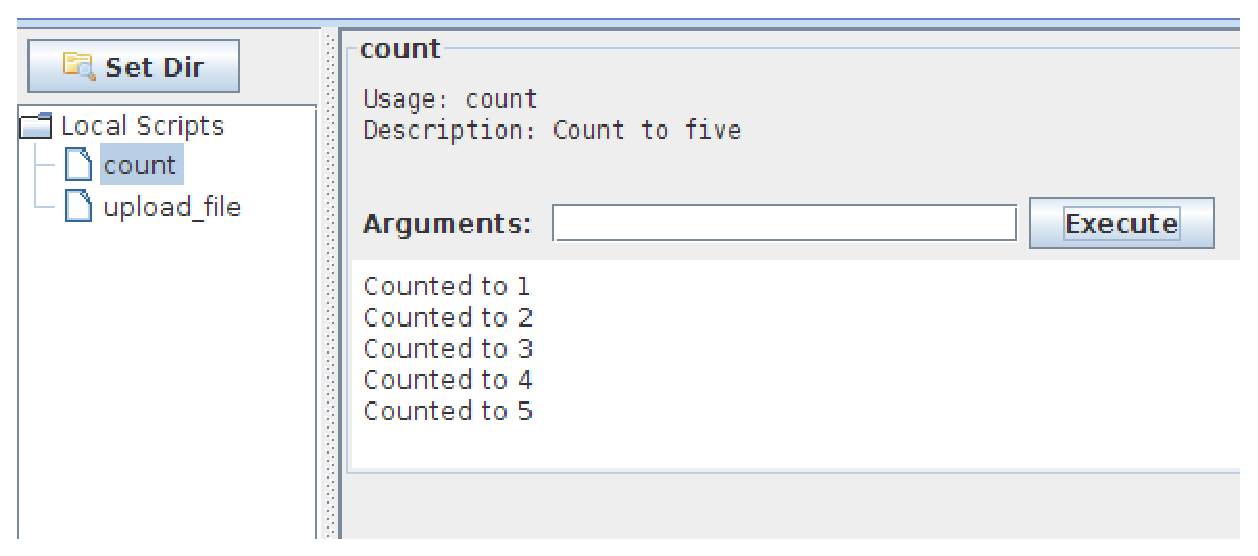
\includegraphics[scale=0.7]{img/fsgui_local}
  \caption{Local Scripts}
\end{figure}

\textbf{Must be able to retrieve a list of server scripts and execute them with custom arguments} \\
FSGui can retrieve a list of available server scripts that the user can choose from. FSServer will implement the available\_scripts command to retreive this information. Once retrieved the GUI builds a tree of the scripts for easy navigation.

When a script has been clicked on in the tree, a script description and a textfield for passing arguments are presented to the user. An execute button will execute the script on the server, any response data will be appended just below the script.

\begin{figure}[h!] \centering
	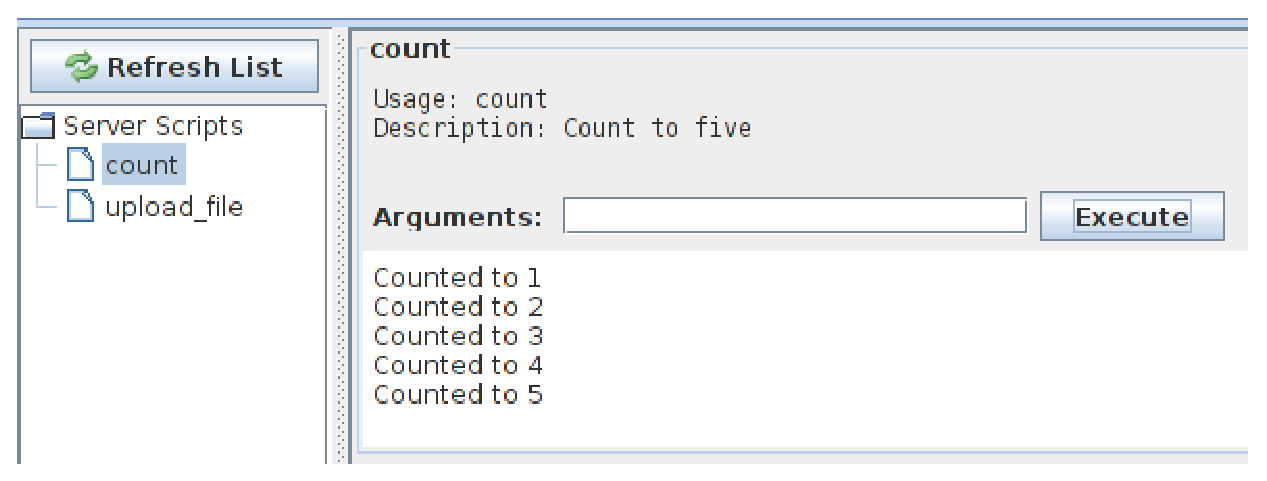
\includegraphics[scale=0.7]{img/fsgui_server}
  \caption{Server Scripts}
\end{figure}

\textbf{Must have an auto\_lock option} \\
An auto\_lock option is available in the connect panel and from the menubar.

\begin{figure}[h!] \centering
	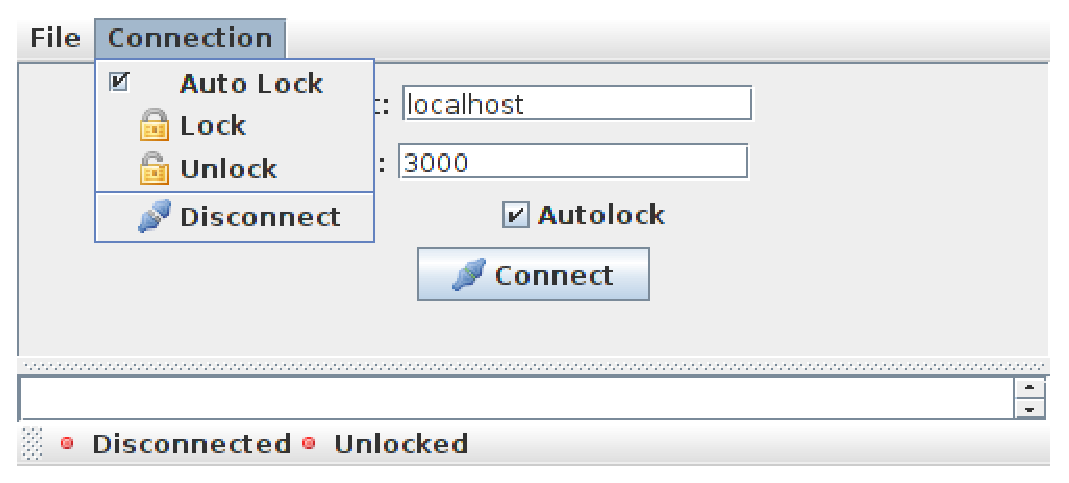
\includegraphics[scale=0.5]{img/fsgui_autolock}
  \caption{Auto Lock, connection and lock status}
\end{figure}

\textbf{Must indicate connection and lock state} \\
There is a statusbar in bottom of the window indicating whether there is a connection or not and whether the server is locked by the gui or not.

\textbf{must indicate when the health status was last updated} \\
In the health panel there is an indication of when the health status was last updated.








\section{Implementation}
Lets look at the non-trivial part of the implementation.

\textbf{FSController} \\
At the heart of the FSGui is the FSController singleton class which is responsible for creating the TCP socket, building the swing gui and setting up the data handlers. Because of its bigbrother like nature it is also extensively used in other classes to reference other parts of the program.

\textbf{Local Scripts} \\
Java has a built-in class called ProcessBuilder that can create a process given a list of the command and its arguments. It will execute and capture the output of the process. We will use this class to execute local scripts.

\textbf{Socket and Socket Callbacks} \\
The built-in class Socket will be used to create the TCP connection and to read/write on the socket. To prevent cluttering in FSController the Socket will be wrapped in a class called FSSocket that will perform callbacks to a class that implements the FSSocketObserver interface when interesting events happen, such as on connection, on disconnection, on incomming data etc. The FSController implements this interface and will therefore be able to act on these events.

\textbf{Data Handlers and request callbacks} \\
When we send a request to the server we will often expect some kind of response. As the solution is push driven we cannot know when the response will come. We cannot send the request and then immediately wait for the response on the socket, potentially throwing away responses to other requests. We have to send the request and just hope that the response will come.

When the response finally do come, we won't know what to do with it. So along with sending a request we most associate it with a callback that should be executed upon a received response.

This is done with a FSCallback which is an interface consisting of one method called onResponse that takes a FSResponse as its parameter. The callback is registered in the requestCallbacks Hashtable where an entriy consists of the requests id as key and the callback as a value.

A class called FSSocketReader will constantly be reading the socket and whenever a message has been read it is first sent to the appropriate data handler and if it is a response, the response handler will look for the id in the requestCallbacks and execute the callback.

When the client gets an incoming message FSGui determines the type of the message and dispatches it to the appropriate data handler. Data handlers must therefore be setup before connecting to the server.

\textbf{The response handler} \\
When sending a request one specifies what piece of code to run when the response is received.
The response handler looks at the id parameter and matches it to the corresponding request and dispatches the data to that piece of code.

\textbf{The token timeout handler} \\
This handler just notifies the user by changing the "locked"-icon in the GUI.

\textbf{JSON Parsing} \\
Java does not have built-in support for JSON, so a third-party library called JSONObject has been used.

\textbf{Generating unique ids for the requests} \\
Unique id generation is handled by FSSocket and is appended the the request before sending it off to the server.
The id should just be an increasing integer as the id-space is limited to each connecting tcp client. The server increments the id in a syncronized method to ensure that only one thread can increment it at a time.

If the id-space was limited to each client, a solution could be to use random numbers. UUIDS are very good to such situations \footnote{A good introduction to UUID's can be found at wikipedia: \texttt{<http://en.wikipedia.org/wiki/Universally\_Unique\_Identifier>} }.

\textbf{Command Sequences} \\
The command sequences are saved in a simple json format. A sequence of the following commands:
\begin{verbatim}
	health_status
	download 0x40000000 512
\end{verbatim}
Will be saved as the following JSON data:
\begin{verbatim}
[
	{"command":"health_status", "arguments":[""]},
	{"command":"download","arguments":["0x40000000","512",""]}
]
\end{verbatim}
NOTE: The empty string in the end of each argument is the options textfield.
